\chapter{Introduction}

On the context of this thesis the motivations that encourage for this work and
the objectives.

\section{Context}
\lettrine{F}{rom} several decades to nowadays the science have been evolving
dramatically in a wide variety of fields, one of the main reasons is because now we
have the technology to provide the enough computational power for face problems
which were typically imposible to solve. The vanguard of this technological
revolution is represented on the huge computers called high performance
computers.
In Computer Science the discipline in charge to drive research in this field is 
the High Performance Computing, i.e. HPC. HPC has been increasing in importance 
and nowadays can be said it is the third support of science with theory and 
mathematics. The science that can be done thanks to this big machines goes from 
earthquake predictions to the analysis of the DNA of a carcinogenic cell, from
weather forecast to material physics simulation.

A typical configuration for high performance machines are clusters. It means a 
team of individual processors or multiprocessors (and lately more specific 
hardware like GPUs) working together, interconnected by a super-fast network. 
The fundamental idea behind these big machines is getting speedup by mean of
partitioning the problem and parallelize the execution. So all processors (or a 
subset) in the cluster will be dealing with different parts of the same problem 
and communicating between them in order to end up with a solution. For example 
imagine we have a weather forecast software, in order to speedup the forecast 
we can partition the surface of the earth and hold every portion to one individual
processor. The communications will be needed because the weather will also depend 
on surroundings, so every partition will need also information of other partitions 
results.

\begin{figure}
  \caption{Gordon Moore's prediction done in 1965}
  \label{moore-prediction}
  \centering
    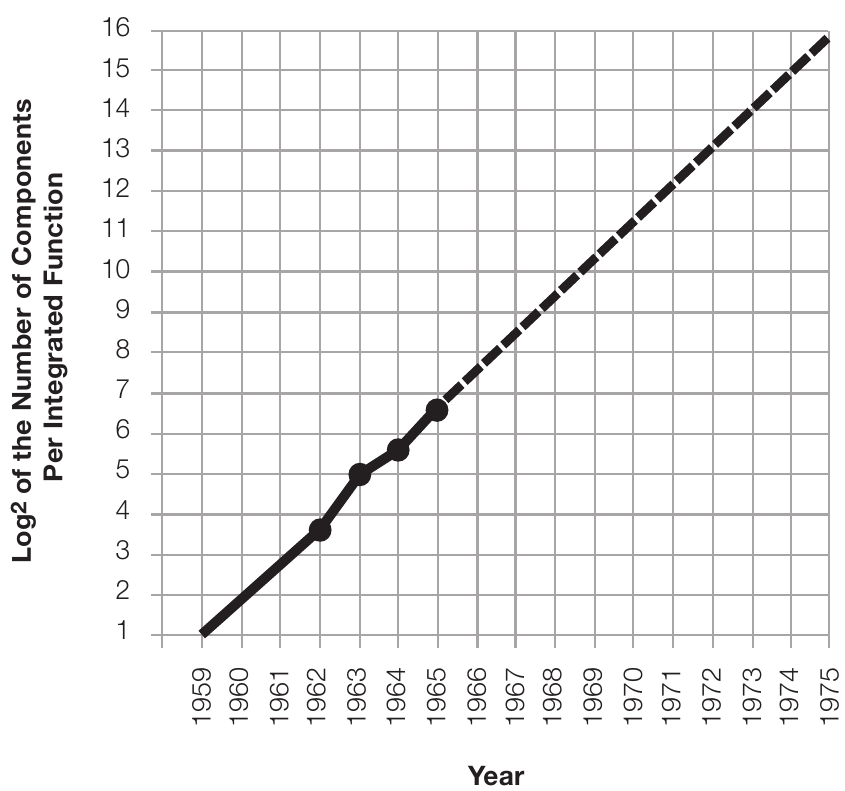
\includegraphics[width=150px]{moore_prediction.png}
\end{figure}


Resources are limited and expensive so we have to use them as efficiently
as its possible. Improving the performance and the efficiency is not just a 
matter that affects to one
layer of the Transformation Hierarchy (proposed by
\cite{transformationHierarchy}, figure \ref{fig:transformation_hierarchy}) 
but can be applied to every one of them. For example the
tremendous evolution of the last fourty years were improvements done mostly on
circuits layer what have been following the Moore's law \cite{moore:1965}. The
manufacturers have been reducing the size of transistors by a ratio of 2 every
18 months as were predicted in figure \ref{moore-prediction}. Performance improvements 
were also at microarchitecture level with
disruptive designs that allows ILP like HPS\footnote{High Performance Substrace,
what is indeed out-of-order execution with in-order retirement.}
\cite{Patt:1985:HNM:18927.18916}, speculative execution with prefetchers, 
branch prediction or even memory access value speculation,
VLIW\footnote{Very Long Instruction Word} or TLP\footnote{Thread Level
Parallelism} with multi-threading. Improvements on memory hierarchy like cache 
associativity, non-blocking cache or trace cache. The last revolution affected 
 microarchitecture, architecture and program layers and was the introduction
of multicores (early 2000s). It is basically a revolution in commodity hardware because HPC
have been used to use shared memory paradigm for a while like for example with
Transputers (1980s). Anyway it is important even in HPC since the trend have
been to move from ad-hoc systems to commodity hardware because the goodnesses of
mass production. On last years researchers have been concerned about the
power consumption because the trend is to have bigger machines so the need of be more
energy efficient is a big deal for the next-generation exascale systems.
Heterogeneity of systems seems to be the trend, i.e. near the typical general
purpose chips install new specific purpose hardware like GPUs or ASICs like
TPUs \cite{jouppi2017datacenter} evolving to an even more complex systems. This
innovation affects to almost all layers of the stack from Program to below. 

\begin{figure}
  \caption{Levels of transformation}
  \label{fig:transformation_hierarchy}
  \centering
    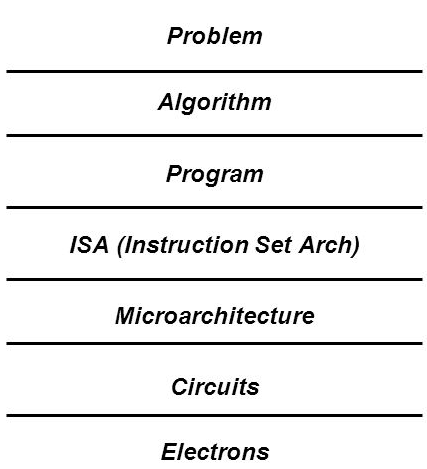
\includegraphics[width=100px]{transformationhierarchy.png}
\end{figure}

Program layer\footnote{The program layer bring together the program itself, 
programming models, frameworks and libraries.} is the interface between pure 
algorithm and the machine architecture. 
It is the actual implementation of the algorithm, i.e. where programmers
transforms algorithm to semantic code that can be transformed lately into
executable binary by compilers. Having an efficient algorithm mathematically 
speaking is not enforcing having an efficient program because at algorithm level 
we do not care about the machine. Pushing on with the business to be always more 
faster and efficient, the tools that aims to this end in program layer are the 
performance analysis tools that allows to detect the bottlenecks presents in the 
application that prevents from better behaviour.

Once the big picture have been briefly introduced now we can zoom in and go a
bit further into details. This thesis belongs to the application performance 
analysis field of research contributing to ease the analysis and the report. 
On the next section a more wide description on performance analysis tools is made.

\subsection{Performance analysis tools}

There are two main trends on analysis tools:
\begin{enumerate}[label=\roman*)]
    \item Profiler tools 
      generates performance summaries that provides coarse-grain information, 
      with low-overhead. It is suitable for these analysis where you do not care
      about the fine grain details so you just want a general overview of the
      behavior of the application.
    \item If your goal is to do a fine-grain analysis more detail is needed. The 
      other typical approach are the tracing tools. High accurate and detailed 
      information can be obtained, but it needs more resources in terms of disk 
      and analyst effort because more data implies more complexity.
\end{enumerate}
There is not a general best choice but is just about the needs. One
disadvantage of profiles is that the high degree of aggregation used to hide
variability, for example if there is the case where one single function
behaves different depending on the phase of the execution. In this direction
research has been drived, e.g. phase-base profiling \cite{malony2005phase} or
CCG \cite{knupfer2005construction}. Other one is
that profilers discard the temporal dimension so the execution sequence is lost.
About the advantages, it is a general summary that allows the user to take a
peek about what is going on, e.g. if the user want to speedup a code a profiler
is a good starting point to figure out where to center the efforts. 

If you look
at tracing tools the obvious advantage is that there is a lot of information
available, in fact with not a lot of effort profiler information can be derived
from traces like is done in Cube \cite{saviankou2015cube}. It can be considered
profiler capabilities as a subset of trace analysis capabilities so there should
be a drawback for tracing because tracing is not always the correct choice. The
main drawback is the scalability for both:
\begin{enumerate*}[label=\roman*)]
  \item In tracing time and
  \item in analysis time.
\end{enumerate*}
The problem is becoming worst since the capacity in 
terms of parallelism is increasing\footnote{As have been said High performance 
computers become more complex every generation, e.g. the current number one on 
the Top500 list is the Sunway TaihuLight with 10,649,600 cores\cite{top500_2017} 
.} so the number of tasks to monitor makes 
tracing techniques by one hand hardly scalable and by the other hand tricky to analyze
because the huge quantity of data and because the increasing response times
during the interactive exploration of analysis results. Researchers are currently 
facing the scalability problems in this two forms. 
There are currently several specialists driving research in the tracing
scalability, they are trying to reduce 
the overhead of tracing in terms of time and trace sizes by mean of several 
techniques like machine learning, data-mining and so on like in 
\cite{llort2015intelligent} or by on-line compression like in
\cite{noeth2009scalatrace}. About analysis time, the complexity of the analysis 
can be overcome by adding some sort of automatization. Some examples of this 
research line are automatic performance analysis \cite{wolf2003automatic}, 
automatic structure extraction \cite{casas2007automatic}, phases detection 
\cite{gonzalez2013application} fundamental factors models \cite{casas2008aass}, 
automatic analysis throw deep learning \cite{simon:2017:perfdp} and so on.
Following to this ambition this thesis is focused on the analysis field and is 
devoted to contribute to ease the work of the analyzers by aid part of the analysis. 

\section{Background}\label{s:pt_evironment}

This thesis has been developed in the Performance Tools team at Barcelona
Supercomputing Center and therefore the developments explained in this
document have been designed to fit in this environment, nevertheless the
techniques are general so could be applied to any other environment.

\subsection{Software}

The main tools designed and developed in the BSC Performance Tools Team are 
Extrae, Paraver and Dimemas although other satellite tools are also in the 
environment they will not be explained because are out of the scope of this 
project. These tools are: 
\begin{enumerate*}[label=\roman*)]
  \item Clustering
  \item Tracking
  \item Folding
  \item Spectral and 
  \item Basic Analysis.
\end{enumerate*}

\subsubsection{Extrae}

Like its name (in spanish) indicates, it is about extracting information. Extrae is
the piece of software in charge of inject monitors to the application to
be studied and
extract valuable information for the analysis. Different mechanism for
monitoring are available being the most used the interposition mechanism by
means of the {\tt LD\_PRELOAD} environment variable present in UNIX systems.
By this mechanism just calls to a given dynamic library can be instrumented because
what it does is to divert shared library calls by the program to extrae, then 
extrae get the information and calls the actual library function. It supports 
several frameworks: 
\begin{enumerate*}[label=\roman*)]
  \item MPI (for several implementations)
  \item OpenMP
  \item OMPSs
  \item CUDA
  \item OpenCL
  \item pThreads
\end{enumerate*}
and virtual machine instrumentation: 
\begin{enumerate*}[label=\roman*)]
  \item Java
  \item and Python.
\end{enumerate*}
The information that can be collected by Extrae is not just timming what is maybe
the most important one but also some hardware counters by means of PAPI
interface. All of this information can be complemented by user events that can
push the desired information to the tracefile by means of the Extrae API. One
possible use of the Extrae API is to extract information about how different
iterations from a given loop are behaving. All these gathered information from 
all threads/processes in the target application is finally merged and presented 
to the analizer as an ASCII tracefile. Since the task of analyze a ASCII file 
is a tough work, a visualizer has been developed, that is Paraver.

The methodology presented in this thesis is about post-mortem trace analysis and
this traces will be generated by extrae so it is an important piece of the
overall workflow. Further Extrae API is used for the validation step in order to
unambiguously detect loops in code and compare the actual structure with the
inferred one automatically without the need of inspect manually the source code.

\subsubsection{Paraver}

The task of analyze raw numbers is tough so the natural choice is to represent 
them visually since we as humans are very
good understanding visual patterns. For example in mathematics
is usual to use plots. In the field of performance analysis, visualizer tools
also has been developed, having in BSC the Paraver (PARAllel Visualization and
Events Representation) tool that as its name indicates
(in spanish) is  about ``to see''. Paraver allows to have a qualitative global 
perception of the application behavior by visual inspection and then to be able 
to focus on the detailed quantitative analysis of the problems.

Its power lies on two main concepts. The first one is that paraver traces are
semantic agnostics therefore it is provided by auxiliar files called pcf (paraver
configuration file\footnote{Do not confuse with cfg files}) and row\footnote{It 
is called row because it provide names for the rows of the timeline so for the 
space axis} (names configuration file). It allows to extend the tool with
support for new performance data or programming models easily. The second and
more interesting is that the derived calculations from initial metrics from trace is
not hardcoded in the tool but configurable so for example to derive a typical
metric like IPC you should filter number of
instructions by one hand, number of cycles by the other hand and then perfom a
division. This powerful approach give the resposability to the user that can
leads to the ``blank page
syndrome''\footnote{https://en.wikipedia.org/wiki/Writer\%27s\_block\#Blank\_page
\_syndrome} for the not so skiled users. For avoid this
sort of problems the Paraver package provides a set of configuration files of
the most used views that perform all the filters and derivations for you.

Even if paraver is not the most important piece of this thesis workflow is
important to introduce it since Paraver traces is what we use and  there is an
interaction between Paraver and the proposed development in the sense that the
second one is capable to identify and communicate with paraver for show up where
in trace are the detected phases.

\subsubsection{Dimemas}

Like the other tools Dimemas also have a so descriptive name, it means (in
spanish) ``tell me more'' but is fine to use the acronim that is ``DIstributed
MEmory MAchine Simulator''. It is a high-abstracted trace-driven MPI simulator
perfect to perform the called ``what if'' experiments. It is capable to simulate
the interconection network of a distributed memory machine by means of a high
abstracted model that consists on three fundamental parameters:
\begin{enumerate*}[label=\roman*)]
  \item Latency (s) that models the actual latency of the network and also the
    possible overhead because the software stack before arrives to the NIC
  \item Bandwidth (mb/s) that models the bandwidth of the network and
  \item Contention that is modeled by the number of messages in flight 
    allowed on a given instant on a given network (intra-nodes, inter-nodes or
    inter-machines) and the number of input and output messages from a given
    node in a given instant.
\end{enumerate*}

Dimemas as Paraver is Extrae-dependant software since they need traces to work.
In the Dimemas case it needs to perform a conversion by means of the {\tt
prv2dim} converter in order to ease the simulation. As an output it builds up a
new Paraver trace that can be analyzed as the original. Only communication times 
are simulated through the Dimemas models so CPU times
remain the same on the output tracefile. Even if it is a minor detail, since it
is important to introduce because the usefulness of it for the purposses of this
thesis, actually there is a mechanism to modify CPU burst times. At parsing time
(done by the {\tt prv2dim}) a hardware counter and a coeficient to multiply 
for this it can be specified. Normally the hardware counter is the number of 
cycles and the coeficient is the cycle time. By this way the user is able to 
remove the possible O.S. noise that has affected the original
execution\footnote{Noise intruced by O.S. can be detected in Paraver by a fall 
  of the frecuency. This is becuse cycles counter forms part of the context of
  every process but not the time so whenever a process loss CPU, cycles will not
  be counted until return to execution but time is not stopped although. This
  phenomena implies an increment on the traced cycle time. Take into account
  that is impossible to guarantee a fall on frequency is because O.S. or because
  any other source like DVFS so it works only when we can assume the frequency
of the processor is quite stable.}.

Can be considered that Dimemas is completely orthogonal to this thesis objetives
but have been considered interesting to introduce it since in some situations a
Dimemas simulation will be needed in order to remove noise from trace since
noise affects quite enough to the proposed methodology because it rely on some
scalar values like timing instead of just an ordered sequence of events.

\subsubsection{Mercurium}\label{ss:mercurium}

Blah Blah Blah

\subsection{Analysis workflow}\label{ss:analysis_workflow}

In an application-centric approach, the performance analysis is a cyclic process 
consisting of observing the behaviour of the application so as to hypothesize the 
possible problems that affect its performance and finally translate these 
hypotheses to improvements in the application re-starting the cycle to validate 
them as is depicted in figure \ref{fig:perf_analysis_workflow}. Obviously, the 
less number of iterations of this cycle the less time wasted and it directly 
depends on the quality of the hypothesis that is strongly related with the 
possibilities the analysis tools provides.

\begin{figure}[]
  \centering
  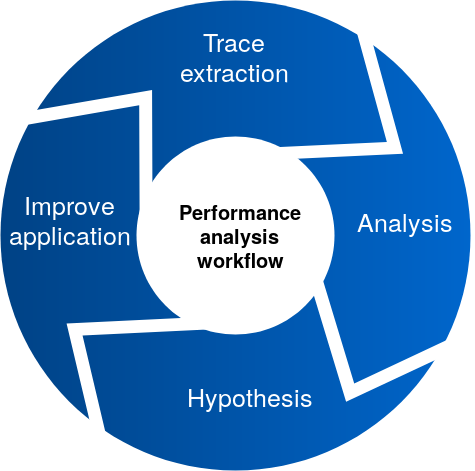
\includegraphics[width=150px]{performance_analysis_diagram.png}
  \caption{Performance analysis workflow}
  \label{fig:perf_analysis_workflow}
\end{figure}

This work is centered on the analysis phase, so lets go further and look at its
subphases. When dealing with little and medium size traces, visualizers used to
be responsiveness enough to perform analysis directly to the traces but when the 
size surpass a given thresshold several previous steps should be done. In last 
cases analysis phase is typically subdivided into the following 
subphases (see figure \ref{fig:analysis_subphases}):
\begin{enumerate}[label=\roman*)]
  \item Filter as much as possible irrelevant information. Before this phase is
    used to be impossible to work with visualizers so the main goal is to end up
    just with the needed information for inspect the structure of the
    application.
  \item HPC applications are used to have a common idiosincracy that is to
    present very repetitive patterns both in space (different processes) and 
    time dimensions. Exploiting this typical characteristic, next step is cut
    the more interesting parts of the execution e.g. an iteration or a set of
    iterations that seems to presents interesting information because its 
    extremelly bad performance.
  \item Last and most important, the inspection. Once one part of the execution is
    detected to be interesting it is then gathered from the original trace i.e.
    with all the original information.
\end{enumerate}

\begin{figure}[]
  \centering
  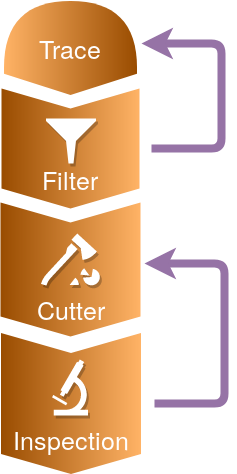
\includegraphics[width=80px]{analysis_subphases.png}
  \caption{Analysis subphases}
  \label{fig:analysis_subphases}
\end{figure}

This work could drive to repeat the same process several times and since every 
one of the steps potentially have a very time consumption, when dealing with
huge trace, it can be a waste of time. 
Both first and second subphases could need to be repeated several times because 
the first filter is not good enough or because on the last phase analyzer realize 
the cut is not as interesting as looked like. The intuition of a high skilled
analyist plays an important role in this process.

As has been covered in motivations (section \ref{s:motivations}) this thesis
approach can be used for improve the inspection subphase but also to help to the
decission or at least give some clues to the analyzer to what region is the most
interesting to cut reducing the number of iterations over the subphases of the
analysis giving more time to the inspection work.

\section{Motivations}\label{s:motivations}

We can say that HPC applications shares a common idiosyncrasy between them. 
Mathematic solvers needs to iterate until the result converge and 
simulation software are used to be programed to evolve over timesteps. So in 
general, HPC applications consists on a big outer loop that is being executed the 
same code but with evolving data, i.e. SPMD\footnote{Single
Program Multiple Data} programs. Additionally this kind of workloads are used
to be burst syncrhonous, i.e. all ranks are executing computation and
communication phases in a syncrhonous manner. For these so regular executions a
relatively simple representation of the whole execution could be extracted, i.e.
the trace could be reduced to a minimum pseudo-code expression
with aggregated data for the whole loop so its somehow folding all the iterations
space. This pseudo-code expresses indeed the actual internal structure of the 
application.

There are several factors that motivates for the extraction of the internal
structure of an application being the most important the first one.


\subsection{About improve understandability of execution}

Even if performance tools have been demonstrated to be valuable on detection of
bottlenecks for a long time, since it demands high skilled profiles for the
analysis, developers are not used to use them but delegate this work to the
actual specialist. One example is the POP programme\footnote{The POP
  (Performance Optimisation and Productivity) center of excellence in computing
  applications provides performance optimisation and productivity services for
academic and industrial codes in all domains. https://pop-coe.eu/}. What it
means is that analyzers are not used to work with its own code so they are used
to be agnostics about the structure of the program and it difficults the process
of relate performance metrics to program code. Having the structure of the
program will lead to better understand the application by allowing to analyzer
to have a mental schema about what the program does and allows to relate
differencies in terms on performance to different program phases. This aid on
the understandability will lead to better and faster analysis while also drives
to better reports to the developer.

There are previous works (discussed widely on section \ref{related_work})  that 
tries to represent the internal structure of an application but they are used to
use directed graphs like in EFG \cite{aguilar2016event} or just callstack trees like
in Cube \cite{saviankou2015cube}. The drawback of represent the application structure
just with directed graphs is that it is a so simplified view, in the referenced
case it is impossible to pinpoint a given loop (directed graph cycle) to the
actual code because the lack of callstack information. In case of the
referenced approach that uses callstacks tree, the lack of information becomes
from the fact that there is no representation for loops (although you have fuzzy
clues like see the number of calls). The identification of this lack of clarity
on the structure representation motivates as well this thesis. The proposal is to 
generate a pseudo-code with loop and conditional structures that can be easily 
pinpointed to source code and additionally can show aggregated metrics so it can 
be understood as a sort of mix of the two approaches references above.

\subsection{About identify regions of
interest}\label{ss:mot_regions_of_interest}

The typical tools like visualizers are not enough responsiveness when dealing
with traces with several GB of information so analyzers needs to first
preprocess the trace before go ahead with the actual inspection. This preprocess
consists basically on filter and cut the trace (widely explained on
\ref{ss:analysis_workflow}) for identify and inspect just these interesting 
hotspots where the bottlenecks seems to be. Automatically extract the structure
of the application will give the possibility to agregate information by phases
and loops so it can aid to analyzer into the work of find out the
hotspots. In this paper \cite{trahay2015selecting} they present an automatic
tool that extract this points automatically based on the criteria that
iterations that behave different from the mean are the interesting ones. The
problem with the approach presented on the cited paper is that the methodology
is difficultly scalable since it presents high complexity and is I/O
intensive since the data should be readed repeatedly and it is a problem
when dealing with big traces. 

\subsection{About be scalable}

Current approaches about extract the intern structure (syntactic but not
behavioral, more details in \ref{related_work}) based on a post-mortem trace
analysis rely on pattern mining techniques (the basic idea of these algorithms 
are exposed on section \ref{pattern_mining}) that is the obvious choice because 
a trace is basically a sequence of events sorted by time. The problem with these 
sort of algorithm is the complexity. So the last motivation is about reducing the 
complexity of this task. The performance of the proposed algorithms are
prohibitive like in \cite{trahay2015selecting} \cite{Safyallah2006}
\cite{Lopez-Cueva2012} so taking into account the exponential increassing of 
traces sizes this thesis contribution is the idea to perform intern structure 
analysis instead of as a pattern mining problem, as a classification problem. 
Classification algorithms like clustering presents about quasy-lineal costs.


\section{Expectations}

The goal of this work is to automatically detect the internal structure of an 
application and correlate it with performance metrics by mean of a post-mortem 
trace analysis that will help to have a general overview about the phases of the 
execution. This will allow the analyst to build up a mental schema about the
application and understand more easily what could be going on. Furthermore it will 
contain source code information that will allow to easly pinpoint one metric to 
the actual code providing an enhacenement on the analyst-developer
understanding. Additionally this structure extraction can help to analyzer to 
decide what part of the trace analyze first since it will allow to know the loops 
and iterations boundaries.

The main objective is to detect those sets of events in trace that are being
repeated toghether several times (above a given threshold) and agrupate them into 
loops. Since several subsets can appear because an application used to have 
dozens of loops, those detected events subsets also will be arranged (in a 
hierarchical manner) in a way that represents faithfully the actual internal 
structure. This sort of analysis have been done tipically by using sequential 
pattern mining techniques what is in principle the set of techniques that better 
fits to this problem since a trace is just a sequence of events ordered by time.

Based on previous works and on the premise that HPC applications used to present
the same idiosincracy (SPMD, burst syncrhonous,\ldots) has been decided to
explore a new way to detect those patters, motivated mainly for the fact that
pattern mining techniques are in general computationally expensive. By using data 
mining clustering techniques we expect to have an scalable
solution since it is used to present quasy-lineal complexity with the number of 
elements to clusterize. The mapping between elements to clusterize and events on
a trace is not bijective but exaustive, so every element potentially represents 
several trace events, what is in fact the same instruction presenting its dynamic
aspect because the execution of loops. Further the reduction of the tracefile
events to the set of elements to clusterize is not needed to be sequential but 
can be done in parallel by spliting the trace into several files and process
them by multiple processes (assuming also multiple HDDs). Assuming repetitive 
executions, the number of elements to clusterize would be about constant despite 
the increasing of the exeuction time.

In this work is not expected to end up with a completelly functional and
performance refined tool but demonstrate how this approach can present valuable 
results with a good scalability on increasing trace sizes.
